\documentclass{beamer}
\usetheme{Madrid}
\usecolortheme{dolphin}
\usepackage{graphicx}
\usepackage{amsmath}
\usepackage{booktabs}
\usepackage{caption}
\usepackage{tikz}
\usepackage{colortbl, tcolorbox}
\usetikzlibrary{shapes.geometric, arrows.meta, positioning}

% Define custom colors for the box background and frame
\definecolor{boxbackground}{rgb}{0.95, 0.95, 0.95}
\definecolor{boxframe}{rgb}{0.0, 0.0, 0.0}

\setbeamertemplate{navigation symbols}{}
\setbeamertemplate{footline}[frame number]

\title[Job Posting Skill Measures]{How Informative are Job Posting Skill Measures?\\Evidence from Selection Decisions}
\author{Nikhil George \and Ramayya Krishnan \and Rahul Telang}
\institute{Carnegie Mellon University}
\date{}

\begin{document}

\begin{frame}
\titlepage
\end{frame}

\begin{frame}{Motivation}
\begin{itemize}
    \item \textbf{Skills-first hiring revolution}
    \begin{itemize}
        \item Google, IBM, Walmart prioritize capabilities over credentials
        \item Reducing emphasis on traditional qualifications
    \end{itemize}
    \item \textbf{Job postings as unvalidated infrastructure}
    \begin{itemize}
        \item Powers algorithms, HR analytics, policy decisions
        \item Assumed to reflect skill demands, but \textcolor{orange}{no validation against outcomes}
    \end{itemize}
    \item \textbf{Stakes are high}
    \begin{itemize}
        \item If uninformative: Undermines billion-dollar HR tech ecosystem
        \item If valid: Unlocks precision in labor markets
    \end{itemize}
\end{itemize}
\end{frame}

\begin{frame}{The Research Gap}
\begin{itemize}
    \item \textbf{Central question:} Do skill measures derived from job postings predict actual hiring decisions?
    \item \textbf{Skepticism about job postings}
    \begin{itemize}
        \item May be aspirational or templated
        \item Could include inflated ``nice-to-have'' skills
    \end{itemize}
    \item \textbf{Critical validation needed}
    \begin{itemize}
        \item Research relies on posting data without outcome validation
        \item HR analytics industry depends on posting informativeness
    \end{itemize}
\end{itemize}
\end{frame}

\begin{frame}{Research Questions}
\begin{enumerate}
    \item Can skill distance measures built on job postings be validated against selection decisions?
    \item How informative are job postings relative to traditional HR metrics?
    \item Can analytics built on job postings reveal new insights about human capital management?
\end{enumerate}
\end{frame}

\begin{frame}{Research Contribution}
\textbf{First Empirical Validation of Job Posting Informativeness}
\begin{itemize}
    \item \textbf{Novel approach}
    \begin{itemize}
        \item Skill distance metric derived solely from job text
        \item Validated against actual selection decisions
    \end{itemize}
    \item \textbf{Unique dataset}
    \begin{itemize}
        \item IT division of major financial firm
        \item 8,180 job postings, 1,370 internal applications
        \item Complete application histories
    \end{itemize}
    \item \textbf{Key findings}
    \begin{itemize}
        \item \textcolor{green}{84\%} higher selection probability for closest skill matches
        \item \textcolor{green}{70\%} of multi-applicant vacancies select closest candidate
        \item Job text outperforms traditional HR metrics (AUC \textcolor{green}{0.62} vs. \textcolor{red}{0.50})
    \end{itemize}
\end{itemize}
\end{frame}

\begin{frame}{A Gap in the Literature}
Prior work focuses on \textcolor{orange}{extraction}, not \textcolor{orange}{validation}:
\begin{itemize}
    \item \textbf{Taxonomy-based approaches} (O*NET, ESCO)
    \begin{itemize}
        \item Static categories, misses contextual nuance
    \end{itemize}
    \item \textbf{Collaborative filtering} (LinkedIn)
    \begin{itemize}
        \item Co-occurrence predictive validity
    \end{itemize}
    \item \textbf{Credential proxies}
    \begin{itemize}
        \item Losing relevance in skills-first hiring
    \end{itemize}
\end{itemize}

\begin{tcolorbox}[colback=boxbackground,colframe=boxframe,sharp corners]
\textbf{Our Breakthrough:} Outcome-grounded validation: Not just what skills are listed, but which ones actually matter
\end{tcolorbox}
\end{frame}

\begin{frame}{Research Setting \& Data}
\begin{itemize}
    \item \textbf{Internal labor market as ideal laboratory}
    \begin{itemize}
        \item Workers move across roles within firm
        \item Can link current job to positions sought
        \item Observe both successful and unsuccessful applications
    \end{itemize}
    \item \textbf{Dataset overview}
    \begin{itemize}
        \item IT division, technology roles with precise requirements
        \item 8,180 job postings (2018--2021)
        \item 1,370 internal applications (650 selected, 720 rejected)
    \end{itemize}
\end{itemize}

\begin{tcolorbox}[colback=boxbackground,colframe=boxframe,sharp corners]
\textbf{Key Advantage:} Ability to measure skill distance between current and target roles
\end{tcolorbox}
\end{frame}

\begin{frame}{Sample Job Postings Comparison}
\begin{columns}
\begin{column}{0.48\textwidth}
\begin{tcolorbox}[colback=boxbackground,colframe=boxframe,sharp corners]
\textbf{Close Match (Selected)}
\begin{itemize}
    \item Position: Data Engineer
    \item Shared skills: Data modeling, ETL, SQL
    \item Distance drivers: Limited architecture experience
\end{itemize}
\end{tcolorbox}
\end{column}
\begin{column}{0.48\textwidth}
\begin{tcolorbox}[colback=boxbackground,colframe=boxframe,sharp corners]
\textbf{Distant Match (Not Selected)}
\begin{itemize}
    \item Position: Full-Stack Developer
    \item Missing skills: Data warehousing, dimensional modeling
    \item Different focus: UI/UX vs. backend data
\end{itemize}
\end{tcolorbox}
\end{column}
\end{columns}

\vspace{0.5cm}
\begin{tcolorbox}[colback=boxbackground,colframe=boxframe,sharp corners]
\centering
\textbf{Box 2.2 Sample Job Description}\\
\small
\textbf{Hadoop developer} for multiple initiatives. Experience in Capacity Planning, Cluster Designing. Develop Big Data Strategy and Roadmap. \\
\textbf{Mandatory Skills:} Hadoop stack (HDFS, MapReduce, Yarn, HIVE, sqoop), Cloudera, NoSQL\\
\textbf{Desired Skills:} Kafka, R, Python, Tableau, Data Lake with Cloudera ecosystem
\end{tcolorbox}
\end{frame}

\begin{frame}{Conceptual Framework}
\begin{itemize}
    \item Job descriptions encode skill requirements that matter for selection
    \item Selection decisions reveal which aspects of postings are most important
    \item Skill alignment between current and target roles predicts outcomes
\end{itemize}

\begin{tcolorbox}[colback=boxbackground,colframe=boxframe,sharp corners]
\textbf{Key Insight:} When an applicant seeks a position that is ``distant'' in required skills from their current job, they have lower probability of being selected
\end{tcolorbox}

\begin{table}
\centering
\begin{tabular}{l c}
\toprule
\textbf{Applicant-Vacancy Skill Distance} & \textbf{Selection Probability} \\
\midrule
Low (close match) & High \\
Medium & Medium \\
High (distant match) & Low \\
\bottomrule
\end{tabular}
\end{table}
\end{frame}

\begin{frame}{Methodological Approach}
\begin{columns}
\begin{column}{0.5\textwidth}
\begin{enumerate}
    \item \textbf{Job Posting Embeddings}
    \begin{itemize}
        \item SBERT model captures semantic richness
        \item 384-dimensional vectors
    \end{itemize}
    \item \textbf{Dimension Reduction}
    \begin{itemize}
        \item PCA + Fuzzy C-Means clustering
        \item Preserves key information
    \end{itemize}
    \item \textbf{Distance Metric Learning}
    \begin{itemize}
        \item Reweights based on priorities
        \item Stretches differentiating dimensions
    \end{itemize}
\end{enumerate}
\end{column}
\begin{column}{0.5\textwidth}
% Placeholder for the figure
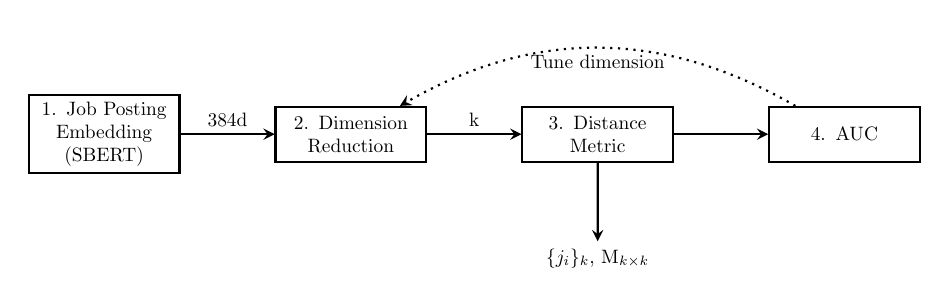
\begin{tikzpicture}[node distance=1.2cm, auto, thick, scale=0.7, every node/.style={scale=0.7}]
    % Styles for boxes and arrows
    \tikzstyle{box} = [rectangle, draw, text width=2.5cm, text centered, minimum height=1cm]
    \tikzstyle{arrow} = [thick,->,>=stealth]
    \tikzstyle{dotted arrow} = [thick,->,>=stealth,dotted]
    
    % Nodes
    \node[box] (embeddings) {1. Job Posting Embedding (SBERT)};
    \node[box, right=of embeddings] (reduction) {2. Dimension Reduction};
    \node[box, right=of reduction] (metric) {3. Distance Metric};
    \node[box, right=of metric] (auc) {4. AUC};
    
    % Text below metric box
    \node[below=1cm of metric] (notation) {\{$j_i$\}$_{k}$, M$_{k \times k}$};
    
    % Arrows
    \draw[arrow] (embeddings) -- node[above] {384d} (reduction);
    \draw[arrow] (reduction) -- node[above] {k} (metric);
    \draw[arrow] (metric) -- (auc);
    \draw[dotted arrow] (auc) to[bend right] node[midway, below] {Tune dimension} (reduction);
    \draw[arrow] (metric) -- (notation);
\end{tikzpicture}
\caption*{Overview of measurement approach}
\end{column}
\end{columns}
\end{frame}

\begin{frame}{Metric Learning: Adapting to Context}
\begin{columns}
\begin{column}{0.48\textwidth}
\begin{itemize}
    \item Distance between jobs $j_c$ and $j_v$:
    \begin{equation}
    d(j_c, j_v; M) = \sqrt{(j_c - j_v)^T M(j_c - j_v)}
    \end{equation}
    
    \item Learn matrix $M$ that:
    \begin{itemize}
        \item Maximizes distance between non-selected pairs
        \item Minimizes distance between selected pairs
        \item Reweights skill dimensions based on historical value
    \end{itemize}
\end{itemize}

\begin{tcolorbox}[colback=boxbackground,colframe=boxframe,sharp corners]
\textbf{Strength: Domain Adaptation}\\
Generic embeddings treat all skills equally, metric learning \textcolor{orange}{tailors to firm context}
\end{tcolorbox}
\end{column}
\begin{column}{0.48\textwidth}
% Placeholder for the figure
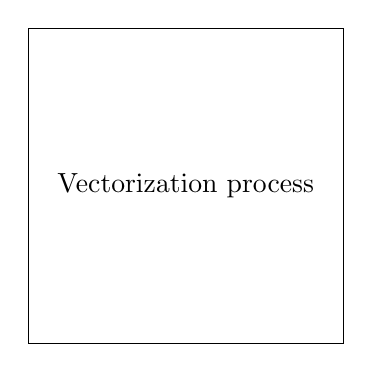
\begin{tikzpicture}
\node at (2,2) {Vectorization process};
\draw (0,0) rectangle (4,4);
\end{tikzpicture}

\begin{tcolorbox}[colback=boxbackground,colframe=boxframe,sharp corners]
\textbf{Limitation: Context Dependency}\\
Reflects historical patterns, could perpetuate biases
\end{tcolorbox}
\end{column}
\end{columns}
\end{frame}

\begin{frame}{Predictive Power of Job Posting Content}
\begin{columns}
\begin{column}{0.48\textwidth}
\begin{table}
\centering
\begin{tabular}{l c l}
\toprule
\textbf{Model} & \textbf{AUC} & \textbf{Interpretation} \\
\midrule
Our approach & \textcolor{green}{0.620} & Significant power \\
SBERT cosine & 0.562 & Some signal \\
HR variables & \textcolor{red}{0.500} & No power \\
\bottomrule
\end{tabular}
\end{table}

\begin{tcolorbox}[colback=boxbackground,colframe=boxframe,sharp corners]
\textbf{Key Finding:}\\
Job posting content has significant predictive power, outperforming traditional HR variables
\end{tcolorbox}

\begin{itemize}
    \item Metric learning adds substantial value over generic embeddings
    \item Selection conditional on application explains limited power of HR variables
\end{itemize}
\end{column}
\begin{column}{0.48\textwidth}
% Placeholder for the figure
\begin{tikzpicture}
\draw[->] (0,0) -- (4,0) node[right] {Dimensions};
\draw[->] (0,0) -- (0,4) node[above] {AUC};
\draw[thick, color=blue] (0.5,1.5) to[out=30, in=180] (2,3) to[out=0, in=150] (3.5,3.2);
\node[right] at (3.5,3.2) {0.62};
\draw[dashed, color=red] (0,2.5) -- (4,2.5);
\node[left] at (0,2.5) {0.50};
\end{tikzpicture}
\caption*{Cross-validated AUC scores across dimensionalities}
\end{column}
\end{columns}
\end{frame}

\begin{frame}{Selection Probability and Skill Distance}
\begin{columns}
\begin{column}{0.45\textwidth}
\begin{tcolorbox}[colback=boxbackground,colframe=boxframe,sharp corners]
\textbf{Key Result:}\\
Selection probability in closest skill distance quintile is \textcolor{green}{84\% higher} compared to furthest quintile
\end{tcolorbox}

\begin{itemize}
    \item Clear monotonic decline across quintiles
    \item Robust to various controls and specifications
    \item Direct evidence of job posting informativeness
\end{itemize}
\end{column}
\begin{column}{0.55\textwidth}
% Placeholder for the figure
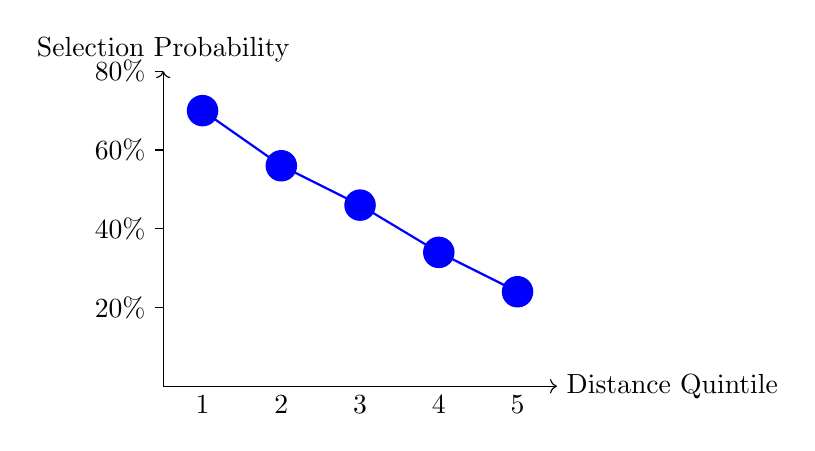
\begin{tikzpicture}
\draw[->] (0,0) -- (5,0) node[right] {Distance Quintile};
\draw[->] (0,0) -- (0,4) node[above] {Selection Probability};
\foreach \x/\y/\lab in {0.5/3.5/1, 1.5/2.8/2, 2.5/2.3/3, 3.5/1.7/4, 4.5/1.2/5} {
    \fill[blue] (\x,\y) circle (0.2);
    \node[below] at (\x,0) {\lab};
}
\draw[thick, blue] (0.5,3.5) -- (1.5,2.8) -- (2.5,2.3) -- (3.5,1.7) -- (4.5,1.2);
\foreach \y/\lab in {1/20\%, 2/40\%, 3/60\%, 4/80\%} {
    \draw (0,\y) -- (-0.1,\y) node[left] {\lab};
}
\end{tikzpicture}
\caption*{Selection Probability by Skill Distance Quintile}
\end{column}
\end{columns}
\end{frame}

\begin{frame}{Causal Evidence from Quasi-Experiments}
\begin{columns}
\begin{column}{0.48\textwidth}
\begin{tcolorbox}[colback=boxbackground,colframe=boxframe,sharp corners]
\textbf{Within-Vacancy Comparisons}
\begin{itemize}
    \item 261 vacancies with multiple applicants
    \item \textcolor{green}{70\%} select candidate with shortest distance
    \item \textcolor{red}{35\% lower odds} per quintile increase in distance
\end{itemize}
\end{tcolorbox}
\end{column}
\begin{column}{0.48\textwidth}
\begin{tcolorbox}[colback=boxbackground,colframe=boxframe,sharp corners]
\textbf{Within-Applicant Comparisons}
\begin{itemize}
    \item 33 applicants with multiple applications
    \item \textcolor{red}{50\% lower odds} for more distant roles
    \item Controls for individual traits
\end{itemize}
\end{tcolorbox}
\end{column}
\end{columns}

\vspace{0.3cm}
\begin{table}
\centering
\begin{tabular}{l l}
\toprule
\textbf{Design} & \textbf{Controls For} \\
\midrule
Within-Vacancy & Vacancy-specific factors (role, team, timing) \\
Within-Applicant & Applicant-specific factors (quality, experience) \\
\bottomrule
\end{tabular}
\end{table}

\vspace{0.2cm}
\begin{center}
\large Skill distance \textcolor{orange}{causally} impacts selection
\end{center}
\end{frame}

\begin{frame}{Skill Distance Shapes Job Search Behavior}
\begin{columns}
\begin{column}{0.48\textwidth}
\textbf{High-distance Applicants}
\begin{itemize}
    \item Apply to \textcolor{green}{1.5x more roles}
    \item More exploratory search
    \item \textcolor{red}{33.5\% lower} selection odds
\end{itemize}

\textbf{Low-distance Applicants}
\begin{itemize}
    \item More targeted applications
    \item Higher success rates
    \item Often more passive in search
\end{itemize}
\end{column}
\begin{column}{0.48\textwidth}
% Placeholder for the figure
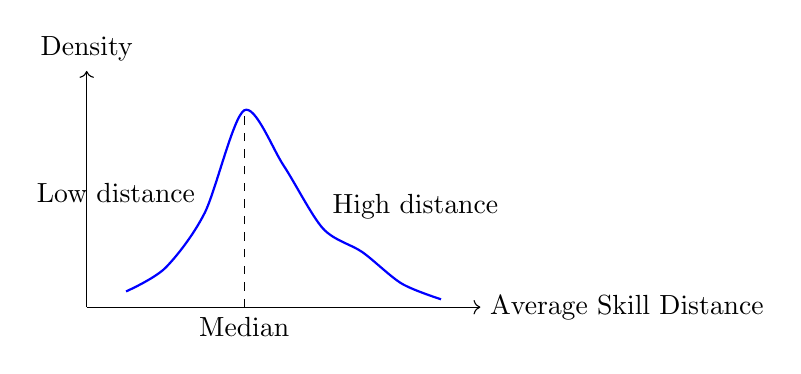
\begin{tikzpicture}
\draw[->] (0,0) -- (5,0) node[right] {Average Skill Distance};
\draw[->] (0,0) -- (0,3) node[above] {Density};
\draw[thick, blue, smooth] plot coordinates {
    (0.5,0.2) (1,0.5) (1.5,1.2) (2,2.5) (2.5,1.8) (3,1.0) (3.5,0.7) (4,0.3) (4.5,0.1)
};
\draw[dashed] (2,0) -- (2,2.5);
\node[below] at (2,0) {Median};
\node[above left] at (1.5,1.2) {Low distance};
\node[above right] at (3,1.0) {High distance};
\end{tikzpicture}
\caption*{Distribution of Average Skill Distance}
\end{column}
\end{columns}
\end{frame}

\begin{frame}{Bridging Theory and Practice}
\begin{columns}
\begin{column}{0.48\textwidth}
\textbf{Theoretical Contributions}
\begin{itemize}
    \item Validates job postings as informative signals
    \item Advances skills-based labor market theories
    \item Addresses information asymmetry
\end{itemize}
\end{column}
\begin{column}{0.48\textwidth}
\textbf{Practical Applications}
\begin{itemize}
    \item Internal mobility recommendations
    \item Targeted skill development
    \item Evidence-based succession planning
\end{itemize}
\end{column}
\end{columns}

\begin{table}
\centering
\begin{tabular}{l l}
\toprule
\textbf{Research Domain} & \textbf{Contribution} \\
\midrule
Labor Economics & Validates key data source, quantifies skill distance \\
HR Analytics & Provides framework for mobility analysis \\
NLP/ML & Demonstrates domain adaptation of language models \\
\bottomrule
\end{tabular}
\end{table}
\end{frame}

\begin{frame}{Methodological Innovation}
\begin{tcolorbox}[colback=boxbackground,colframe=boxframe,sharp corners]
\textbf{Prior Assumptions:}
Job postings are aspirational or generic, best analyzed with one-size-fits-all models
\end{tcolorbox}

\begin{tcolorbox}[colback=boxbackground,colframe=boxframe,sharp corners]
\textbf{Our Approach:}
Learn from real selection decisions what aspects of postings actually matter
\end{tcolorbox}

\begin{table}
\centering
\begin{tabular}{l l}
\toprule
\textbf{Challenge} & \textbf{Our Solution} \\
\midrule
Generic embeddings miss context & Metric learning adapts to organization \\
``Noise'' in job descriptions & Selection decisions reveal what matters \\
Historical biases in hiring & Focus on predictive validity, not prescription \\
\bottomrule
\end{tabular}
\end{table}

Framework is generalizable to other domains requiring context-specific language interpretation
\end{frame}

\begin{frame}{Conclusion}
\begin{itemize}
    \item First validation against real decisions: Job postings are highly informative
    \item Outperforms traditional HR metrics (AUC \textcolor{green}{0.62} vs. \textcolor{red}{0.50})
    \item Informativeness maximized by combining generic embeddings with firm-specific outcomes
\end{itemize}

\begin{tcolorbox}[colback=boxbackground,colframe=boxframe,sharp corners]
\textbf{Opens New Lens on Labor Markets}
\begin{itemize}
    \item Skill distance shapes search behavior and outcomes
    \item Enables data-driven workforce strategies
    \item Strengthens case for skills-first hiring approaches
\end{itemize}
\end{tcolorbox}

Our validation transforms job postings from static text into a dynamic, validated signal for labor market decisions
\end{frame}

\begin{frame}
\centering
\huge Thank You!

\vspace{2em}
\Large Questions?

\vspace{2em}
\normalsize Contact: nikhilg@cmu.edu
\end{frame}

\end{document}